\documentclass[10pt, conference]{IEEEtran}
\usepackage[english]{babel}
\usepackage[utf8]{inputenc}
\usepackage[usenames]{color}
\usepackage{colortbl}
\usepackage{comment}
\usepackage{graphicx}
\usepackage{epsfig}
\usepackage{array, colortbl}
\usepackage{listings}
\usepackage{epstopdf}
\usepackage{multirow}
\usepackage{rotating}
%\usepackage{subfigure}
\usepackage{subfig}
\usepackage{float}
\usepackage[obeyspaces,hyphens,spaces]{url}
\usepackage{balance}
\usepackage{fancybox}
\usepackage{scalefnt}
\usepackage[normalem]{ulem}
%\pagestyle{plain}
\pagenumbering{arabic}
\pagestyle{empty}
\clubpenalty = 10000
\widowpenalty = 10000
\displaywidowpenalty = 10000
\usepackage{cleveref}

\makeatletter
\renewcommand{\paragraph}[1]{\noindent\textsf{#1}.}

\title{Ton Du Langage: Une Analyse De La Relation Entre Les Émotions Et L'Issue De La Compilation}
\author{Antoine Gagné, Olivier Grenier-Chénier}

\begin{document}
\maketitle

\begin{abstract}
Dans un contexte où les programmes et applications évoluent rapidement, l'industrie de développement logiciel encourage l'utilisation d'outils d'intégration continue tels que Travis CI. L'organisation de l'International Conference on Mining Software Repositories met à la disposition des chercheurs une base de données, nommée TravisTorrent, mettant en lien des commits de dépôt Github avec leur succès ou échec de compilation. Afin d'explorer de nouvelles avenues de Data Mining, la présente étude s'intéresse au lien entre le type de langage et les émotions véhiculées dans les commentaires associés aux pull requests et le succès ou échec de compilation par Travis.
\end{abstract}


\section{Introduction}
\label{sec:introduction}
Dans l’industrie du développement logiciel, appliquer un processus d’intégration continue (continuous integration) est généralement admis comme une bonne pratique \cite{c3}. Grâce en partie à son intégration avec GitHub, la plateforme Travis CI est considérée par plusieurs comme étant la plus efficace et la plus répandue dans le domaine des logiciels libres. Cependant, peu d’études empiriques ont été effectuées sur les bienfaits de cette plateforme. C’est le défi que propose la conférence internationale sur l’extraction de données des dépôts (repository) de logiciel, ou International Conference on Mining Software Repositories \cite{c2} en anglais. Cette organisation fournit au grand public un volumineux ensemble de données relatives aux différents aspects de compilation logiciel (TravisTorrent) et encourage tous les intéressés à l’étudier afin d’en déceler les potentielles tendances ou corrélations cachées qui pourraient élargir l’éventail des connaissances du domaine. 


\section{Question de recherche}
\label{sec:rq}
L’avenue que nous avons tenté d’explorer par rapport à ce défi est axée sur l’aspect psychologique des développeurs. Nous avons tenté de déterminer si le “ton” des commentaires liés à un commit a une influence statistiquement significative sur le succès d’une compilation. On entend ici par “ton” l’ensemble des sentiments et émotions évoqués par les conversations des développeurs lorsque ces derniers discutent et débattent sur les forums de leur projet GitHub. On cherche à savoir si certains éléments, si certaines formulations utilisées ou façons de s’exprimer qu’ont les développeurs a un impact sur le fait qu’un commit compile avec succès ou non. Pour faire cette analyse sémantique des commentaires, nous avons utilisé une application offerte par IBM appelée Tone-Analyser de la suite d’applications Bluemix. Cette application, alimentée par le moteur cognitif Watson, permet de déceler trois types de tons dans un texte : les émotions, le comportement social et le style du langage. Plus de détails sur les données retournées par l'API Bluemix peuvent être trouvées à \cite{c1}. \\
Ainsi, la question de recherche explorée ici est: “Existe-il un lien entre le ton utilisé dans les dépôts github et la passation des tests de Travis?”

\section{Défis techniques}
\label{sec:Defis}
Ce travail a posé plusieurs défis importants. D'abord, les données de TravisTorrent en lien aux différentes compilations sont assez volumineuses et ne sont pas toutes pertinentes à l'analyse à souhaitons effectuer. En effet, seules les lignes des données ayant un nombre élevé de commentaires permettent d'avoir des échantillons suffisamment fiables afin d'en retirer les sentiments qui y sont prédominants. Cela consistait en une tâche plus compliquée que prévu car, après avoir effectué une analyse plus approfondie des données de TravisTorrent, nous avons remarqué qu'il existait des incohérences entre les informations des données et celles transmises par l'API de GitHub. Bien qu'il soit possible de connaître le nombre de commentaires associés à un commit par les données de TravisTorrent, nous avons remarqué que ces données ne sont pas toujours exactes. Après investigation, il semble qu'il existe des cas où les données TravisTorrent indiquent qu'un certain nombre de commentaires soient associés à un certain commit, mais que l'API de GitHub nous indique qu’il n’y en a pas. Le cas inverse est aussi possible, il existe des cas où les données TravisTorrent affirment qu'aucun commentaire n'est associés à un commit alors que l'API GitHub retourne des commentaires pour ce commit. Dans le but d’utiliser les meilleurs données possible, certaines informations fournies par TravisTorrent ont donc été ignorées afin de privilégier celles de GitHub. \\
Un autre obstacle à prendre en compte était les limites imposées par les deux API à utiliser. L'API de GitHub permet un maximum de 5000 requêtes par heure. L'API de Bluemix est plus contraignant, et impose un maximum de 1000 requêtes gratuites par mois, puis le modèle devient payant. Cela nous a donc forcé à faire faire l’analyse de ton par fil de commentaire plutôt que par commentaire. \\
Finalement, les résultats dépendent directement de la précision et de l'efficacité de l'application Tone-Analyser de BlueMix, puisqu'il n'est bien évidemment pas possible de faire cette analyse de ton manuellement et sans biais cognitif. Cela pose un risque à la fiabilité des résultats, vu le nombre élevé de termes techniques, d’hyperliens, d'abréviations et autres à prendre en compte lors de l’analyse. 


\section{Méthodologie}
\label{sec:Methodologie}
L’acquisition de données est réalisée en 5 étapes : \emph{A)} L’acquisition des commentaires via l’API de Github, \emph{B)} l’appariement des données Github avec les données TravisTorrent, \emph{C)} le filtrage des données données Github et TravisTorrent et \emph{D)} l’acquisition des données d’analyse de ton de Bluemix. L’analyse \emph{E)} est quant à elle accomplie en testant la corrélation entre les analyses de Bluemix et le succès ou l’échec de la compilation par TravisTorrent.

\subsection{Acquisition des commentaires Github}
Chaque ligne du fichier TravisTorrent contient des données permettant de faire le lien avec les dépôts GitHub telles que le nom du projet, les identifiants correspondant aux commits traités par TravisTorrent, le numéro du pull request (si applicable) ainsi que le nombre de commentaires associés à ces commits. \\
Voici la méthodologie utilisée. D'abord, afin d'éviter d'avoir un trop gros ensemble de données et de respecter la limite de 5000 requêtes par heure imposée par L'API de GitHub, seuls les projets ayant au moins 10 développeurs et ayant au moins 10000 lignes de codes ont été considérés, ce qui donne un sous-ensemble de 135 projets, répartis sur 1026891 lignes du fichiers TravisTorrent. Ensuite, les commentaires associés à ces projets ont été récupérés via l'API de GitHub. Ces commentaires sont répartis en 3 catégories, les commentaires sur le dépôt (endpoint /comments), les commentaires associés à des lignes spécifiques de code (endpoint /pulls/comments) et les commentaires associés au pull request même (endpoint /issue/comments) \cite{c4}. À noter que pour GitHub, chaque pull request est un issue en soi, d'où l'endpoint commençant par /issue/. Pour ces requêtes, l’API retourne tous les commentaires liés au pull request, à l’exception du commentaire original. Les commentaires originaux ont donc été omis de l’analyse, car les obtenir un par un aurait demandé trop de requêtes. \\
Les commentaires n’étant pas retournés tout d’un bloc, ils sont regroupés à partir des données reçues, puis séparés d’une étiquette \textless COMMENT\textgreater. Voir l’exemple en Annexe A.

\subsection{Appariement des données Github aux données TravisTorrent}
Dans le JSON retourné par l'API, on retrouve les identifiants des commits ainsi que le numéro des pull requests auxquels sont associés les commentaires. Avec ces informations, il est possible d’effectuer une recherche dans les données TravisTorrent afin de trouver les observations  correspondant aux informations reçues de l'API. En passant par l’API Github plutôt que d’utiliser les données TravisTorrent comme base permet d’obtenir des données dont la provenance est plus sûre. Puisque certaines entrées du fichiers de données de TravisTorrent ne comportent pas de commentaires, cette opération a permis de garder 256251 lignes sur les 1026891 du fichier filtré. 

\subsection{Filtrage des données Github et TravisTorrent}
Les fils de commentaires obtenus ont été filtrés afin d’en obtenir moins de 1000, dans le but de pouvoir les envoyer à l’API Bluemix. Pour ce faire, seuls les commentaires associés à des pull requests dans les données TravisTorrent ("gh\_is\_pr"), seuls ceux associés à des dépôts notés comme étant du Ruby et seuls ceux ayant été obtenus par l’API endpoint /issue/comments ont été gardés. Étant donné la structure du TravisTorrent, les commentaires appartenant à des pull requests dont les tests ont été roulés pour différents environnements apparaissent en multiples exemplaires, pour dire si les tests associés à chaque environnement a passé. Les duplicatas ont été éliminés. \\
L’Annexe B contient un exemple de fil de commentaire tel qu’envoyé en entrée à Bluemix.

\subsection{Acquisition des données d’analyse de ton de Bluemix} 
Cette étape a été réalisée en utilisant l’API Bluemix recueillir l’analyse de ton des fils de commentaires. L’endpoint utilisé est situé à https://gateway.watsonplatform.net/tone-analyzer/api/v3/tone en passant le paramètre "version":"2016-05-19". Une fois ces analyses obtenues, elles sont appariées aux commits du TravisTorrent correspondants. \\
Les données de ton retournées par Bluemix contiennent, pour le document entier ainsi que par phrase, une analyse émotionnelle, sociale et de langage. Dans ce projet, seul les émotions associées à l'ensemble du document sont analysées. En tout, les 13 données suivantes sont retournées sous forme de nombre entre 0 et 1 : Joy, Fear, Sadness, Disgust, Anger, Openness, Concientiousness, Extraversion, Agreeableness, Emotional Range, Analytic, Confidence et Tentative. Une portion de donnée retournée est fournie en exemple en annexe B. Les détails de chaque élément peuvent être retrouvés sur le site web de l'application \cite{c1}

\subsection{Analyse}
Les données compilées sont ensuite analysées via Python, spécifiquement la librairie statsmodels (version 0.6.1). La librairie statsmodels contient une fonction Logit (Logistic Regression) qui permet de tester un modèle logistique pour la donnée binaire d’intérêt, dans ce cas-ci Build pass/fail, nommée "tr\_status" dans les données.
Afin de fournir un deuxième type d’analyse, les données sont également passées dans un générateur d’arbre (J48) avec Weka \cite{c5}. Encore une fois, "tr\_status" est fournie comme variable dépendante. 


\section{Resultats}
\label{sec:resultats}

\begin{figure}[t]
  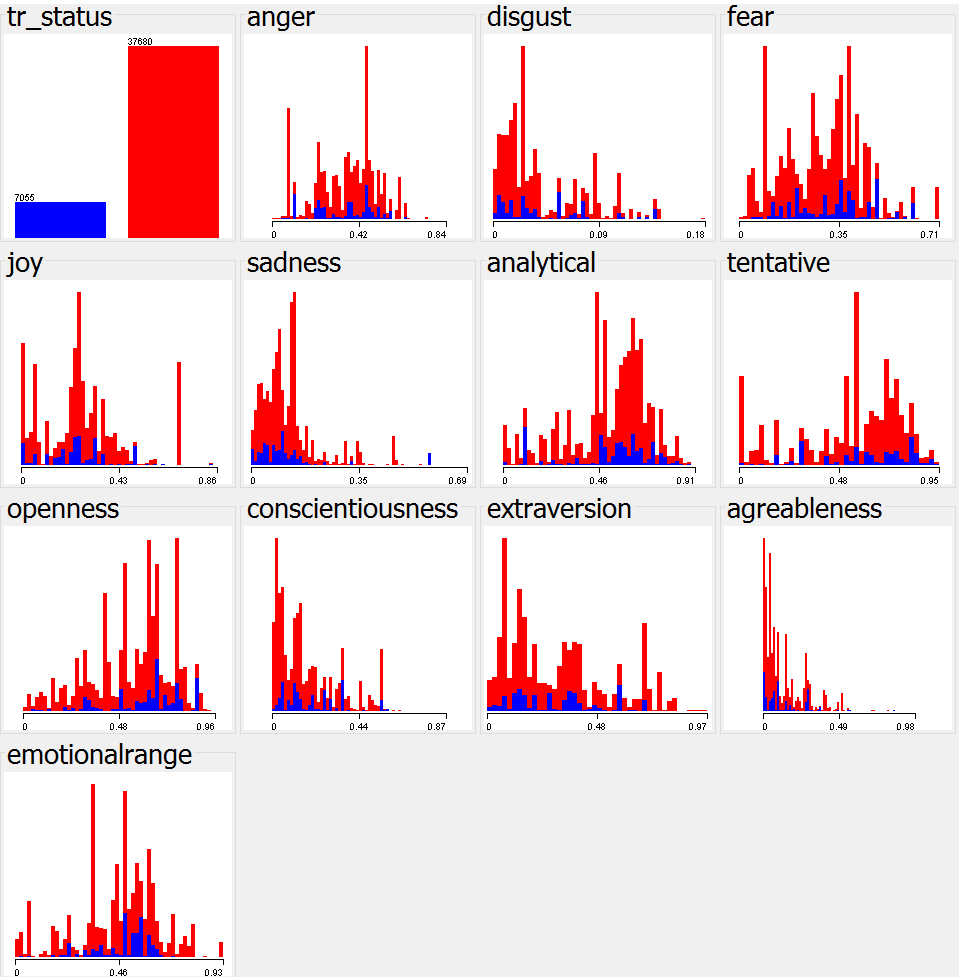
\includegraphics[width=\linewidth]{wekahisto.png}
  \caption{Histogrammes de distribution des sentiments}
  \label{fig:weka1}
\end{figure}

\begin{figure}[t]
  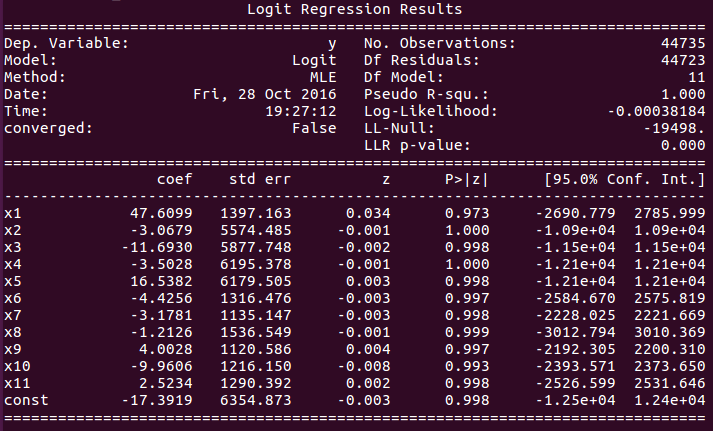
\includegraphics[width=\linewidth]{logit.png}
  \caption{Arbre décisionnel J48}
  \label{fig:logit}
\end{figure}

\begin{figure}[t]
  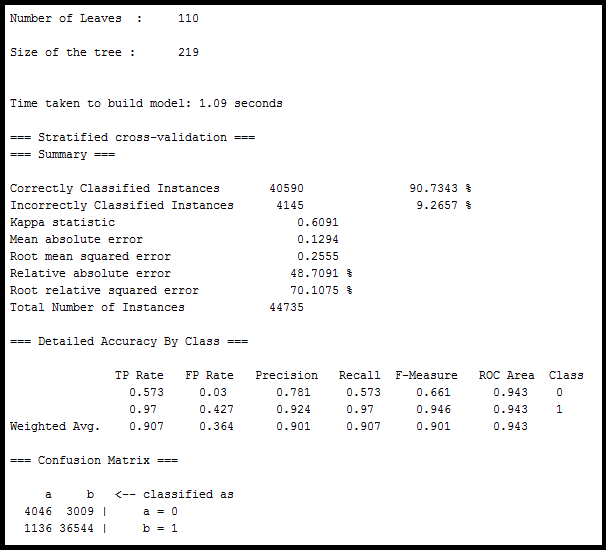
\includegraphics[width=\linewidth]{wekaresult.png}
  \caption{Arbre décisionnel J48}
  \label{fig:weka2}
\end{figure}

Les histogrammes retournés par Weka sont montrés à la figure \ref{fig:weka1}. Leur analyse qualitative ne révèle aucune tendance particulière permettant de discriminer entre un test échoué et réussi. Il apparait comme quoi certaines distributions sont légèrement différentes l'une de l'autre, sans toutefois qu'il n'y ait de séparation ou de pattern clair.

L’analyse par régression logistique (Logit) donne les résultats affichés à la figure \ref{fig:logit}. Les lignes x1 à x11 représentent, dans l’ordre : anger, fear, joy, sadness, tentative, openness, conscientiousness, extraversion, agreableness, emotionalrange. Dans tous les cas, les z-values sont très faibles. Toute forme de corrélation est donc à exclure. 

L’analyse par arbre J48 sur Weka, quant à elle, retourne le résultat de la figure \ref{fig:weka2}. Bien que les résultats semblent plus prometteurs (ROC Area de 0.943), le nombre de feuilles (109) et la taille de l’arbre (219) permet de douter de l’applicabilité réelle de l’arbre. En effet, il semble qu'il s'agisse plutôt d'un cas d'"overfitting" \cite{c6}. Recalculer l'arbre à partir des paramètres discrétisés via un "Unsupervised Discretize" de Weka donne un résultat similaire.


\section{Discussion}
\label{sec:discussion}

Une analyse statistique a permis d’exclure la possibilité de corrélation entre les données fournies par Bluemix et l'issue de la compilation sur Travis. Cependant, plusieurs facteurs peuvent influencer ce résultat.
Premièrement, l’utilisation même de Bluemix est à considérer comme source d’erreur, car n’ayant pas accès à un barème clair sur la manière de catégoriser le langage, il faut faire confiance à leur algorithme. \\
Deuxièmement, l’utilisation d’un langage comprenant de nombreux mots avec une sémantique particulière au domaine (e.g. Pull request, Github, Stack), des acronymes (e.g. PR, Repo, LMK - let me know) rend plus difficile la tâche d’analyse de ton. De plus, de nombreux commentaires contiennent des hyperliens, des codes de référence à des bugs, des dates abrégées (On Fri, Sep 5, 2014), etc… ce qui ne fait pas de sens dans le contexte d’une analyse de langage naturel. \\
Finalement, à cause des nombreux codes, hyperliens et autres technicalités, l’algorithme Bluemix avait fréquemment de la difficulté à identifier le début et la fin des phrases et analysait parfois comme une seule phrase des textes écrits par deux interlocuteurs différents. À cause de la taille du rapport, aucun exemple n’est fourni, mais chaque phrase analysée par Bluemix est retournée avec un score, et il arrive fréquemment de voir une phrase analysée qui contient un segment d’une première phrase et le début d’une deuxième. \\
À cause de tous ces éléments, il n'apparaît pas comme impossible qu’une relation entre le ton et le succès ou échec d’une compilation ait été dissimulé par le “bruit”, bien que cela semble improbable vu les z-values extrêmement bas observés dans la régression logistique. \\

\section{Travail futur}
\label{sec:future}

Trois voies sont à envisager pour améliorer le concept:
La première est d’améliorer l’algorithme décrit précédemment en:
\begin{itemize}
\item Enlevant les blocs de code et stacktrace des commentaire uniquement conserver les commentaires en langage “naturel” des développeurs.
\item Éliminant/développant les acronymes.
\item Remplaçant le langage naturel en un équivalent naturel.
\item Effectuant l’analyse commentaire par commentaire, ou reformater le fil de commentaires de manière à bien identifier les changements de phrases et d’interlocuteur.
\end{itemize}
La seconde est de changer le type de données brute utilisée comme source pour l’analyse. Ainsi il serait intéressant d’utiliser des mailing list de développement ou conversations sur Slack, Hangouts ou autre en lien avec des bugs. Dans ces cas, il sera plus difficile de lier ces informations avec les succès de compilation, mais le langage utilisé risque d’être plus naturel, permettant une analyse plus fiable par Bluemix. \\
Finalement, il serait intéressant d'accomplir la même étude mais avec d'autres langages de programmation. Dans le but de limiter le nombre d'appels D'API à Bluemix à moins de 1000, seulement les dépôts écrits en "Ruby" ont été gardés, mais il serait intéressant d'utiliser cette analyse pour voir si différents langages produisent des résultats différents. Pour aller dans une direction légèrement différente, il serait envisageable de comparer le type d'émotions véhiculées entre les développeurs de différents langages.

\section{Conclusion}
\label{sec:conclusion}

En conclusion, une analyse des commentaires sur les pull requests de Github par l'API tone-analyzer de Bluemix a été effectuée pour en extraire les tons et émotions. En faisant correspondre ces données à TravisTorrent pour mettre en relation le succès des compilation aux émotions, le test de régression logistique n'a pas pu montrer de relation. De plus, l'arbre J48 calculé était trop complexe pour être un modèle réaliste. Ces résultats tendent à montrer qu'il n'existe pas de relation entre le ton des développeurs dans les commentaires de pull request et le succès ou échec de leur compilation. Cependant, plusieurs facteurs viennent mitiger cette conclusion, et une expérimentation approfondie est nécessaire avant de conclure définitivement qu'il n'existe pas de lien entre les émotions véhiculées dans les commentaires et le succès des compilations par Travis. 

\balance

\begin{thebibliography}{1}
\bibitem{c1} Tone Analyzer Service Documentation (Octobre 2016) IBM, En ligne \emph{http://tex.stackexchange.com/questions/3587/how-can-i-use-bibtex-to-cite-a-web-page} 
\bibitem{c2} Conference on Mining Software Repositories (Octobre 2016) MSR, En ligne \emph{http://2016.msrconf.org/\#/home} 
\bibitem{c3} Vasilescu, B. and al., (2015) Quality and Productivity Outcomes Relating to
Continuous Integration in GitHub, \emph{Joint Meeting on Foundations of Software Engineering}
\bibitem{c4} GitHub Developper (Octobre 2016) GitHub, En ligne \emph{https://developer.github.com/v3/} 
\bibitem{c5} Classification Methods (Octobre 2016) University of Minnesota Duluth, En ligne \emph{http://www.d.umn.edu/~padhy005/Chapter5.html} 
\bibitem{c6} Overfitting in Decision Trees (Octobre 2016), University of Notre Dame, En ligne \emph{http://www3.nd.edu/~rjohns15/cse40647.sp14/www/content/lectures/24\%20-\%20Decision\%20Trees\%203.pdf} 
\end{thebibliography}

\end{document}
